\section{Related Work}
\label{sec:relatedWork}

The research gathered from the SLR will form the foundation of the thesis, and this Section is the results of the final data synthesis, all describing a vehicle routing problem attempted solved by a swarm inspired method. 

%\newline
%----------------------------- solving VRPs using swarm intelligence using car transirtation

\subsection{Research Solving VRPs involving cars}

Many computer scientists has since then studied the possibility of solving VRPs using swarm intelligence. \citet{hsiao04}, \citet{salehi-nezhad07}, \citet{tripathi09}, \citet{salehinejad10} and \citet{sedighpour14} all studied the possibility of using swarm intelligence to solve vehicle routing problems involving cars transporting either persons or goods.

%Mangler informasjon om algoritmene som sammenlignes med. Parametersettingen er beskrevet, men ikke forklart. 
\citet{hsiao04} presented an approach to search for the best path of a map considering the traffic loading conditions. To do this, they proposed an ACO algorithm to search for the shortest path from a desired origin to a desired destination. The presented algorithm is a classic ACO algorithm without changes, and compared their algorithm to a brute method emphasizing on the time used to generate the route. Their results states that if the map consists of more than 200 nodes, the ACO performs better than a brute method. In fact, they found that the more nodes the map contains, the higher the benefit of using the ACO algorithm. 

\citet{salehi-nezhad07} presented an ant algorithm to search for the best path between two desired  intersections in cities, called Ant-based Vehicle Navigation algorithm. To get more accurate results than the classic ant algorithms they employed an \textit{awarding/punishment}-method, were the path found by the ``best ants'' are given more pheromone than the path of the ``bad ants''. In order to find the best path, the presented algorithm is concerned about the parameters \textit{distance}, \textit{width}, \textit{traffic load}, \textit{road risk}, \textit{road quality}, and \textit{number of intersections}. The importance of each of the parameters are weighted from 0 to 1 by the user. \emph{\color{blue} Hvordan gikk det med denne?}

%Mangler informasjon om algoritmene som sammenlignes med
\citet{tripathi09} solved the vehicle routing problem with stochastic demand, in which the customer demand is modeled as a stochastic variable. They performed this using an improved version of the ACO approach, called ns-AAA SO. The proposed algorithm orients the search progressively towards favoring the global optimal solution. To do this they defines that a complete iteration consists of two tours: The first tour is a social tour that corresponds to a standard ACO iteration. The second tour is a neighborhood tour where the ants are allowed to communicate important information found in the social tour and change their solutions. If the fitness value of the new solution is better, the old solution found in the social tour is replaced. To favor the optimal solution, the path of the global best path is given more pheromones. Further, to prevent the search from entrapment into a local optima, a minimum quantity of pheromone on any edge, $t_{min}$, is always maintained. The performance of ns-AAA SO was compared with both a standard ACO algorithm and a genetic algorithm. They found that ns-AAA SO outperforms the other two algorithms in every problem instance described by the authors.

%Mandler informasjon om parametersetting
%\citet{dias14} introduced an inverted ACO (IACO) algorithm. The idea is that the IACO algorithm inverts the logic of the classical ACO algorithm by converting the attraction of ants towards pheromones into a repulsion effect. The proposed approach was used in a decentralized traffic management system, where the drivers acted as the inverted ants. The drivers were repelled by the scent of pheromones (other drivers), and the system thus avoids congested roads. The described approach was compared to a shortest-time algorithm (ST), and the IACO algorithm performs better than the ST algorithm with the respect to trip time, travel length, fuel consumption and $CO_2$ emissions. This is as long as a considerable amount (25-50\%) of the vehicles uses the inverted ant algorithm to decide which road to choose. 

%Parameterne er nevnt og den sammenligner med relevante algoritmer.
\citet{salehinejad10} introduced a route selection system which uses an ant colony system to detect an optimum multiparameter direction between two desired points in urban areas. Their algorithm is called Fuzzy Logic-Ant Colony System (FLACS), and like \citet{tripathi09} the pheromone updating is conducted in two parts. First the ants leave pheromone as they walk along a path (local pheromone update rule), and second the global best ant's path is given extra pheromone to favor the global best solution (global pheromone update rule). FLACS differs from other ACSs by the employment of fuzzy logic for the local pheromone updating. The system is concerned about the parameters ``Distance'', ``Traffic Flow'', and ``Incident Risk'' on each edge. FLACS also implements a tabu list, where visited nodes are added to avoid cycles. The algorithm is applied to a part of London, United Kingdom, consisting of 42 junctions. The FLACS algorithm is compared to a standard ACS-algorithm and a $A^*$-ACS-algorithm emphasizing on the parameters mentioned above. They found that FLACS performs better at average than both the standard ACS and the $A^*$-ACS regarding operational cost, regardless of the importance rate of the parameters. It is, however, worth mentioning that the estimation of further traffic data is done by ANNs, and therefore the traffic data used for each algorithm is not exactly the same.They found that FLACS has less running time than $A^*$-ACS, but more than the standard ACS due to its Fuzzy Logic system component. 

%Sammenligner ikke algoritmen mot original ACO, selvom de sier at de ønsker å forbedre ACO i introduksjonen
\citet{sedighpour14} introduced a hybrid ACO (HACO) algorithm to solve the open vehicle routing problem (OVRP). This is a sub problem of the classical VRP where the vehicles are not required to return to the depot. To overcome some of the shortcomings of the original ACO, such as slow computing speed and local convergence, they made three major improvements. First they equipped each node with a candidate list containing nodes nearby that had not yet been visited. Second, at each iteration, they applied several local search techniques to the \textit{n} best solutions found to improve them further. Third, they decided the amount of released pheromone based on the rank of the best known solution found so far. The HACO algorithm was compared with three versions of PSO (standard PSO, PSO without one-point move (PSOWO) and PSO without neighbors (PSOWN) regarding performance. The algorithms were tested on fifteen different sets, consisting of 19 to 72 nodes with 2 to 7 vehicles fixed at the minimum possible. Their result table shows that HACO performs better than the others regardless of the test case used.
\newline

\subsection{Research Solving UTNDP}

Urban Transit Network Design Problem (UTNDP), a subproblem of VRP, considers other objectives and requires other methods for generating solutions than classical VRP problems. As mentioned in Section \vref{sec:VRP}, is UTNDP divided in two parts. The first part includes creating urban transit routes on existing networks (UTRP) and the second part involves the development of schedules (UTSP). The aim of UTRP is generally to minimize the average trip time by maximizing the number of direct travelers per unit lengths. \citet{yang07}, \citet{salehinejad10}, \citet{jiang10}, \citet{poorzahedy11}, \citet{nikolic14}, and \citet{kechagiopoulos14} all addressed problems related to the UTNDP.

%Parameterne er nevnt, men ikke begrunnet. Sammenligner med relevante algoritmer. 
\citet{jiang10} describes an improved ACO (IACO) algorithm to solve the UTRP. The specific improvement made to the algorithm is the implementation of a stagnation counter to determine whether the algorithm has fallen into stagnation. When there is no better solution found after an iteration, the stagnation will increase by 1. When the stagnation counter reaches a certain threshold, the pheromone levels associated with each edge is reinitialized. This improvement is done to compensate for the classical ACOs shortcomings of easily falling into stagnation and therefore obtain a local optimal solution. The IACO algorithm is, like the algorithm described by \citet{yang07}, compared to the classical MMAS algorithm. The results shows significant improvement to the convergence speed compared to MMAS. The also found that IACO performed better both regarding average number of iterations and average path distance. 

%Parameterne er nevnt og den sammenligner med relevante algoritmer
\citet{yang07} presented an optimization algorithm for a urban bus network design (UBND), a problem closely related to the UTNDP. This algorithm is based on \citet{dorigo96}s Ant Colony Algorithm (ACA), called coarse-grain parallel ant colony algorithm (CPACA). CPACA is very similar to the original ACA, but it applies less communication between the ants by dividing the colony of ants into sub colonies that runs in parallel and only communicate with each other. Their results are compared with the classical MAX-MIN ant system (MMAS)\citep{stutzle99} and with ACA with Ant-weight strategy (ACA+). They found that CPACA performs best regarding both average direct traveler density and run time. 

%Parameterne er nevnt, diskutert og begrunnet. Sammenligner for så vidt med relevante algoritme (GA).
\citet{poorzahedy11} proposed an Ant System application for solving the bus network design problem (BNDP). BNDP is defined as the study of choosing a subset of interconnected bus routes among a given set of such routes. A successful solving of the BNDP, like UTNDP, minimizes the total travel time of the users of the network and the operational cost. Like the FLACS algorithm proposed by \citet{salehinejad10}, the proposed AS algorithm also employs a tabu list for each ant where visited nodes are added. Their solution generates multiple nests across the pedestrian network and each nest is responsible for creating a sub network, which is combined to a complete bus network at the end. The algorithm is only concerned about one objective; a combination of travel time for the users and the bus fleet size for the operator. The application was used to design the bus network of Mashhad to further be compared with a genetic algorithm (GA). Their results shows that their algorithm performs better than the GA in both the number of routes, fleet size, in-vehicle travel time and waiting time. Because both the fleet size and number of routes attained by AS is smaller than the ones obtained by GA, GA performs better with respect to travelers walking time. However, both GA and AS performs significantly better than the existing solution on all measures.  

%Parameterne er nevnt, men ikke begrunnet. Sammenligner med relevante algoritmer. 
\citet{nikolic14} proposed a model for solving the UTNDP. To do this they used an improved version of the original BCO \citep{lucic03}. The bees starts with an initial solution at each iteration, where the the initial solution is the best known solution so far. And this initial solution is updated if a better solution is found. The algorithm was tested on Mandl's benchmark problem of a Swiss bus network\citep{mandl80} and compared to competitive approaches (\citet{mandl80}; \citet{shih94}; \citet{baaj95}; \citet{bagloee11}). The performance criteria used to measure the performance was regard to the percentage of total transfer demands satisfied directly ($d_0$), with one transfer ($d_1$), two transfers ($d_2$), or with more than two transfers or not satisfied at all ($d_{unsat}$). The algorithms are also compared regarding average in-vehicle travel time ($ATT$). The experiments are conducted on route set designs with four, six, seven and eight routes. The found that the proposed algorithm performed best regarding total travel time and number of transfers if the order of importance was set to favor what was best for passengers and the number of lines was greater than 4. If the order of importance was set to favor what was best for the operator, the algorithm created the solution with the smallest fleet size independent of number of lines, but then the algorithm performed mediocre regarding all the other measures. 

%Parameterne er nevnt, diskutert og begrunnet. Sammenligner med relevante algoritmer.
\citet{kechagiopoulos14} designed and presented an original PSO algorithm without any changes or improvements. Their goal was to find an efficient solution to the UTRP. The target problem was, like \citet{nikolic14}, Mandl's benchmark problem, and their algorithm was compared with competitive approaches, including genetic algorithms and other metaheuristic approaches mentioned in literature (\citet{baaj91}; \citet{chakroborty02}; \citet{kidwai98}; \citet{fan10}; \citet{fan09-2}; \citet{zhang10}; \citet{chew12}). The algorithms were compared to the same performance criteria and the same amount of route set sizes as \citet{nikolic14}. They found that the proposed algorithm performs better than the competitors regarding $ATT$ independent the route size, and achieves a better percentage of direct travelers ($d_0$) except when the route size is four.  

\subsection{Summary of the Related Work}

Swarm intelligence algorithms has been proven to be useful in many vehicle routing problems, and many studies have been conducted to improve the solution, both regarding time complexity and quality. \citet{dorigo97} and \citet{lucic03} were two of the first published papers that shows methods from swarm intelligence being suitable for solving VRP's. They use respectively an ant colony system and a bee system to solve the Traveling Salesman Problem (TSP), which is a subproblem of VRP. Using methods from swarm intelligence to solve VRP's are still fairly unexplored, and there are many questions to be both asked and answered. However, in the passed decade, there has been published a fare amount of research on the subject, and we believe that research which clearly compares the proposed SI-algorithm to other relevant algorithms increases the credibility of the research and also contributes valuable information to the field. We see that a lot of the newest published research addresses the weaknesses of classical SI-methods and makes changes to the original algorithms to overcome some of these. In these cases we believe that the conducted experiments should include comparison with other swarm inspired methods to indicate whether or not their solution improved the addressed weaknesses. \citet{tripathi09}, \citet{yang07}, \citet{salehinejad10}, and \citet{jiang10} all presented research where their ant colony inspired algorithms were designed to overcome some of the known weaknesses, such as getting stuck at local optima. They compared their solutions with other corresponding swarm methods, achieving promising results. Because of this comparison, they are able to concretely say whether or not the addressed weaknesses are improved. \citet{sedighpour14} also improved the classic ACO to overcome slow computational speed and local convergence. However \citet{sedighpour14} did not compared the proposed algorithm to other implementations of ACO, and the research will not be valid to conclude whether or not it actually overcomes some of ACO's weaknesses. \citet{poorzahedy11} does not test their solution against other swarm intelligence methods, but against the reasonable GA algorithm. The comparison against a GA in the research is descriptive, because they did not add additional features to the AS algorithm. \citet{salehi-nezhad07} did not compare their algorithm against any other algorithm at all, which makes their results hard to verify. 

The performance of metaheuristic methods, including swarm inspired methods, are highly dependent on their parameter settings. The process of parameter tuning is an important contribution to the field of swarm intelligence in general. Multiple researches, including \citet{salehi-nezhad07} and \citet{yang07}, describes their parameter setting as a product of ``trial and error''. We consider this to be a weakness of their research, and therefore not feasible to replicate and compare with. \citet{sedighpour14}, \citet{poorzahedy11}, and \citet{kechagiopoulos14} discussed and justified their parameter settings by conducting their experiments in two parts; one for parameter setting and one for performance. \citet{hsiao04}, \citet{salehi-nezhad07}, \citet{tripathi09}, \citet{sedighpour14}, \citet{yang07}, \citet{salehinejad10}, \citet{jiang10}, \citet{poorzahedy11}, \citet{nikolic14}, and \citet{kechagiopoulos14} all describes the parameters used by their algorithm. This makes their experiments feasible to replicate and compare against.  

The size of the test cases used are an important factor for determining both scalability and robustness of the proposed algorithm. \citet{nikolic14} and \citet{kechagiopoulos14} both uses Mandl's benchmark problem as input. This benchmark problem, presented in Fig. \vref{fig:MandlNetwork_problemstatement},  is a small network containing 15 nodes and 21 edges.  Mandl's network is widely used and acknowledged by multiple researchers, including \citet{baaj91}, \citet{chakroborty02}, and \citet{fan09}. We believe this is a strength of their researches, because this enables them to compare their results to a numerous of other solutions using the same benchmark problem. However, as mentioned, the Mandl network is quite small. We believe that the robustness of their algorithms regarding both time and space complexity could have been verified by also applying their algorithm to a larger test case. \citet{salehi-nezhad07} also applied their solution to a small test set, containing only 27 intersections and requiring only 5 ants and, like the authors that used the Mandl Network, we believe the robustness could have been verified by also applying the algorithm to a larger test set.  \newline

%Regarding our research question \ref{itm:1a}, we conclude after this literature review that swarm intelligence methods are suitable for solving vehicle routing problems.
\subsection{Answering Research Questions}

After a structured review of the related work we can conclude that swarm intelligence methods are suitable for solving vehicle routing problems, and with this answer our research question \vref{itm:1a}. \citet{tripathi09}, \citet{dias14}, \citet{poorzahedy11}, \citet{nikolic14}, and \citet{kechagiopoulos14} all compared their algorithm against other approaches than SI and found that the proposed SI-algorithms generally performed better.

It seems that the state-of-the-art of solving vehicle routing problems using swarm intelligence methods (research question \vref{itm:1b}) can be summed up to as being inspired by the original SI-algorithms, but to add and remove features to make the algorithm more suited for the tasks. With respect to research question \vref{itm:1c}, ten out of the twelve reviewed papers made changes to the original algorithm and the specific changes are described above. We notice a trend of implementing a notion of the best known solution so far, and using this to either directly or indirectly improve the solutions created by the individuals of the swarm (\citet{tripathi09}; \citet{sedighpour14}; \citet{nikolic14}). Due to this, the implementation of this feature in ACO and BCO approaches is, to the best of our knowledge, the only attempt to combine different SI methods (Research Question \vref{itm:1d}). 

\subsection{Problem Statement}
\label{sec:problemStatement}

The goal with this research is to optimize the bus network in Trondheim in order to increase the number of public transportation passengers. The current solution of Trondheim' bus network, managed by AtB\citep{website:atb}, consist of an experience based route network. This means the transit routes are not properly, computationally optimized concerning the travel demand and travel time. In order to contribute to this, we will in this thesis create a swarm intelligence inspired algorithm for the UTRP. A good route network will ensure that routes having the most traveling demands are satisfied with short paths and few vehicle transfers, making travel demand a key variable for the algorithm. AtB does not possess accurate data about the travel demand, and detailed investigations into measuring and predicting travel demand is a complex research problem, beyond the scope of this thesis. Demand values and travel times are all provided for Mandl's benchmark problem\citep{mandl79}. For the UTRP, Mandl's benchmark problem is widely used, whereas a recognized metric is established for evaluating the performance. Due to the reasons stated above, Mandl's benchmark problem will be used as the input data, comparing our results with regard to the acknowledged performance criteria\citep{nikolic14,kechagiopoulos14} (Research Question \vref{itm:2b1}). The comparison will also determine the performance of the algorithm. 

As mentioned, changes to the classic ACO is widely done to overcome some of the algorithm's known weaknesses.  Research Question \vref{itm:2a} is concerned about whether or not it is efficient to add attributes from other swarm intelligence methods in order to improve ACO's computational results. The trend in adding a notion of the best known solution to ACO shows improved performance. In BCO, the artificial bees use a similar approach in rewarding best solutions. We will therefore investigate in building on this best known solution feature with respect to how BCO operates. \citet{kechagiopoulos14} used a PSO algorithm which proved to perform better than all solutions compared to. Due to this, we will also investigate adding possible features from PSO in order to improve the performance of ACO further. 

We did not manage to find any previous research that used graph databases in combination with the vehicle routing problem and swarm intelligence (Research Question \vref{itm:3a}). As mentioned in \vref{subsubsec:neo4j}, does the graph database Neo4j \citep{website:neo4j} have several advantageous features for managing graphs, and we will therefore determine potential advantages and disadvantages of using Neo4j in our implementation and in the optimization process, giving us research question \vref{itm:3b}.

%To determine the effectiveness of the algorithm, will the new proposed algorithm's results be compared to results published in similar research \citep{kechagiopoulos14}, \citep{mandl79}, \citep{fan09}, \citep{nikolic14}, giving Research Question \vref{itm:2b1}.  

As mentioned, the goal with the implementation that it further can be used to optimize Trondheim's transit network. This goal cannot be fully answered until it is applied to the city, but we will strive to create a method that is easily adaptable with the concerns of public transportation in cities in mind. Research Question \vref{itm:2c}, is concerned whether or not it is possible to apply the proposed algorithm to optimize urban transit routes in real urban cities. To do this the algorithm will be implemented in a way that it is easily adaptable to new input values, and it will be tested on large networks more similar to real transit networks. 

%The current solution of AtB consist of an experience based route network, and therefore not properly, computationally optimized concerning the travel demand and travel time. When a route network is not properly optimized, it can lead to a large number of transfers for passengers when they are traveling from their origin to their destination, resulting in a long total travel time. A good route network will ensure that routes having the most traveling demands are satisfied with short paths and few vehicle transfers, making travel demand a key variable for the algorithm. AtB\citep{website:atb} does not possess accurate data about the travel demand, and detailed investigations into measuring and predicting travel demand is a complex research problem, and beyond the scope of this thesis. Demand values and travel times are all provided for Mandl's benchmark problem\citep{mandl79}, and will in this thesis be used as the input data. For the urban transit routing problem (UTRP), Mandl's network seems to be the only benchmark instance used and acknowledged by researchers\citep{kechagiopoulos14},\citep{nikolic14}. The algorithms from these papers are, and the proposed algorithm in this thesis will be compared with regard the same performance criteria and route set sizes.

%As seen in \citet{hsiao04}, the classical ACO has several advantages for the VRP, such as natural parallelism and continuous positive feedback, which allows good solutions to be identified fast. However, ACO also has a few drawbacks including the weakness of getting stuck at a local optima. We will investigate the possibility of overcoming this drawback and to enhance the optimization process, by improving ACO, and including features from other swarm inspired methods. 

\begin{figure}[H]
\begin{center}
  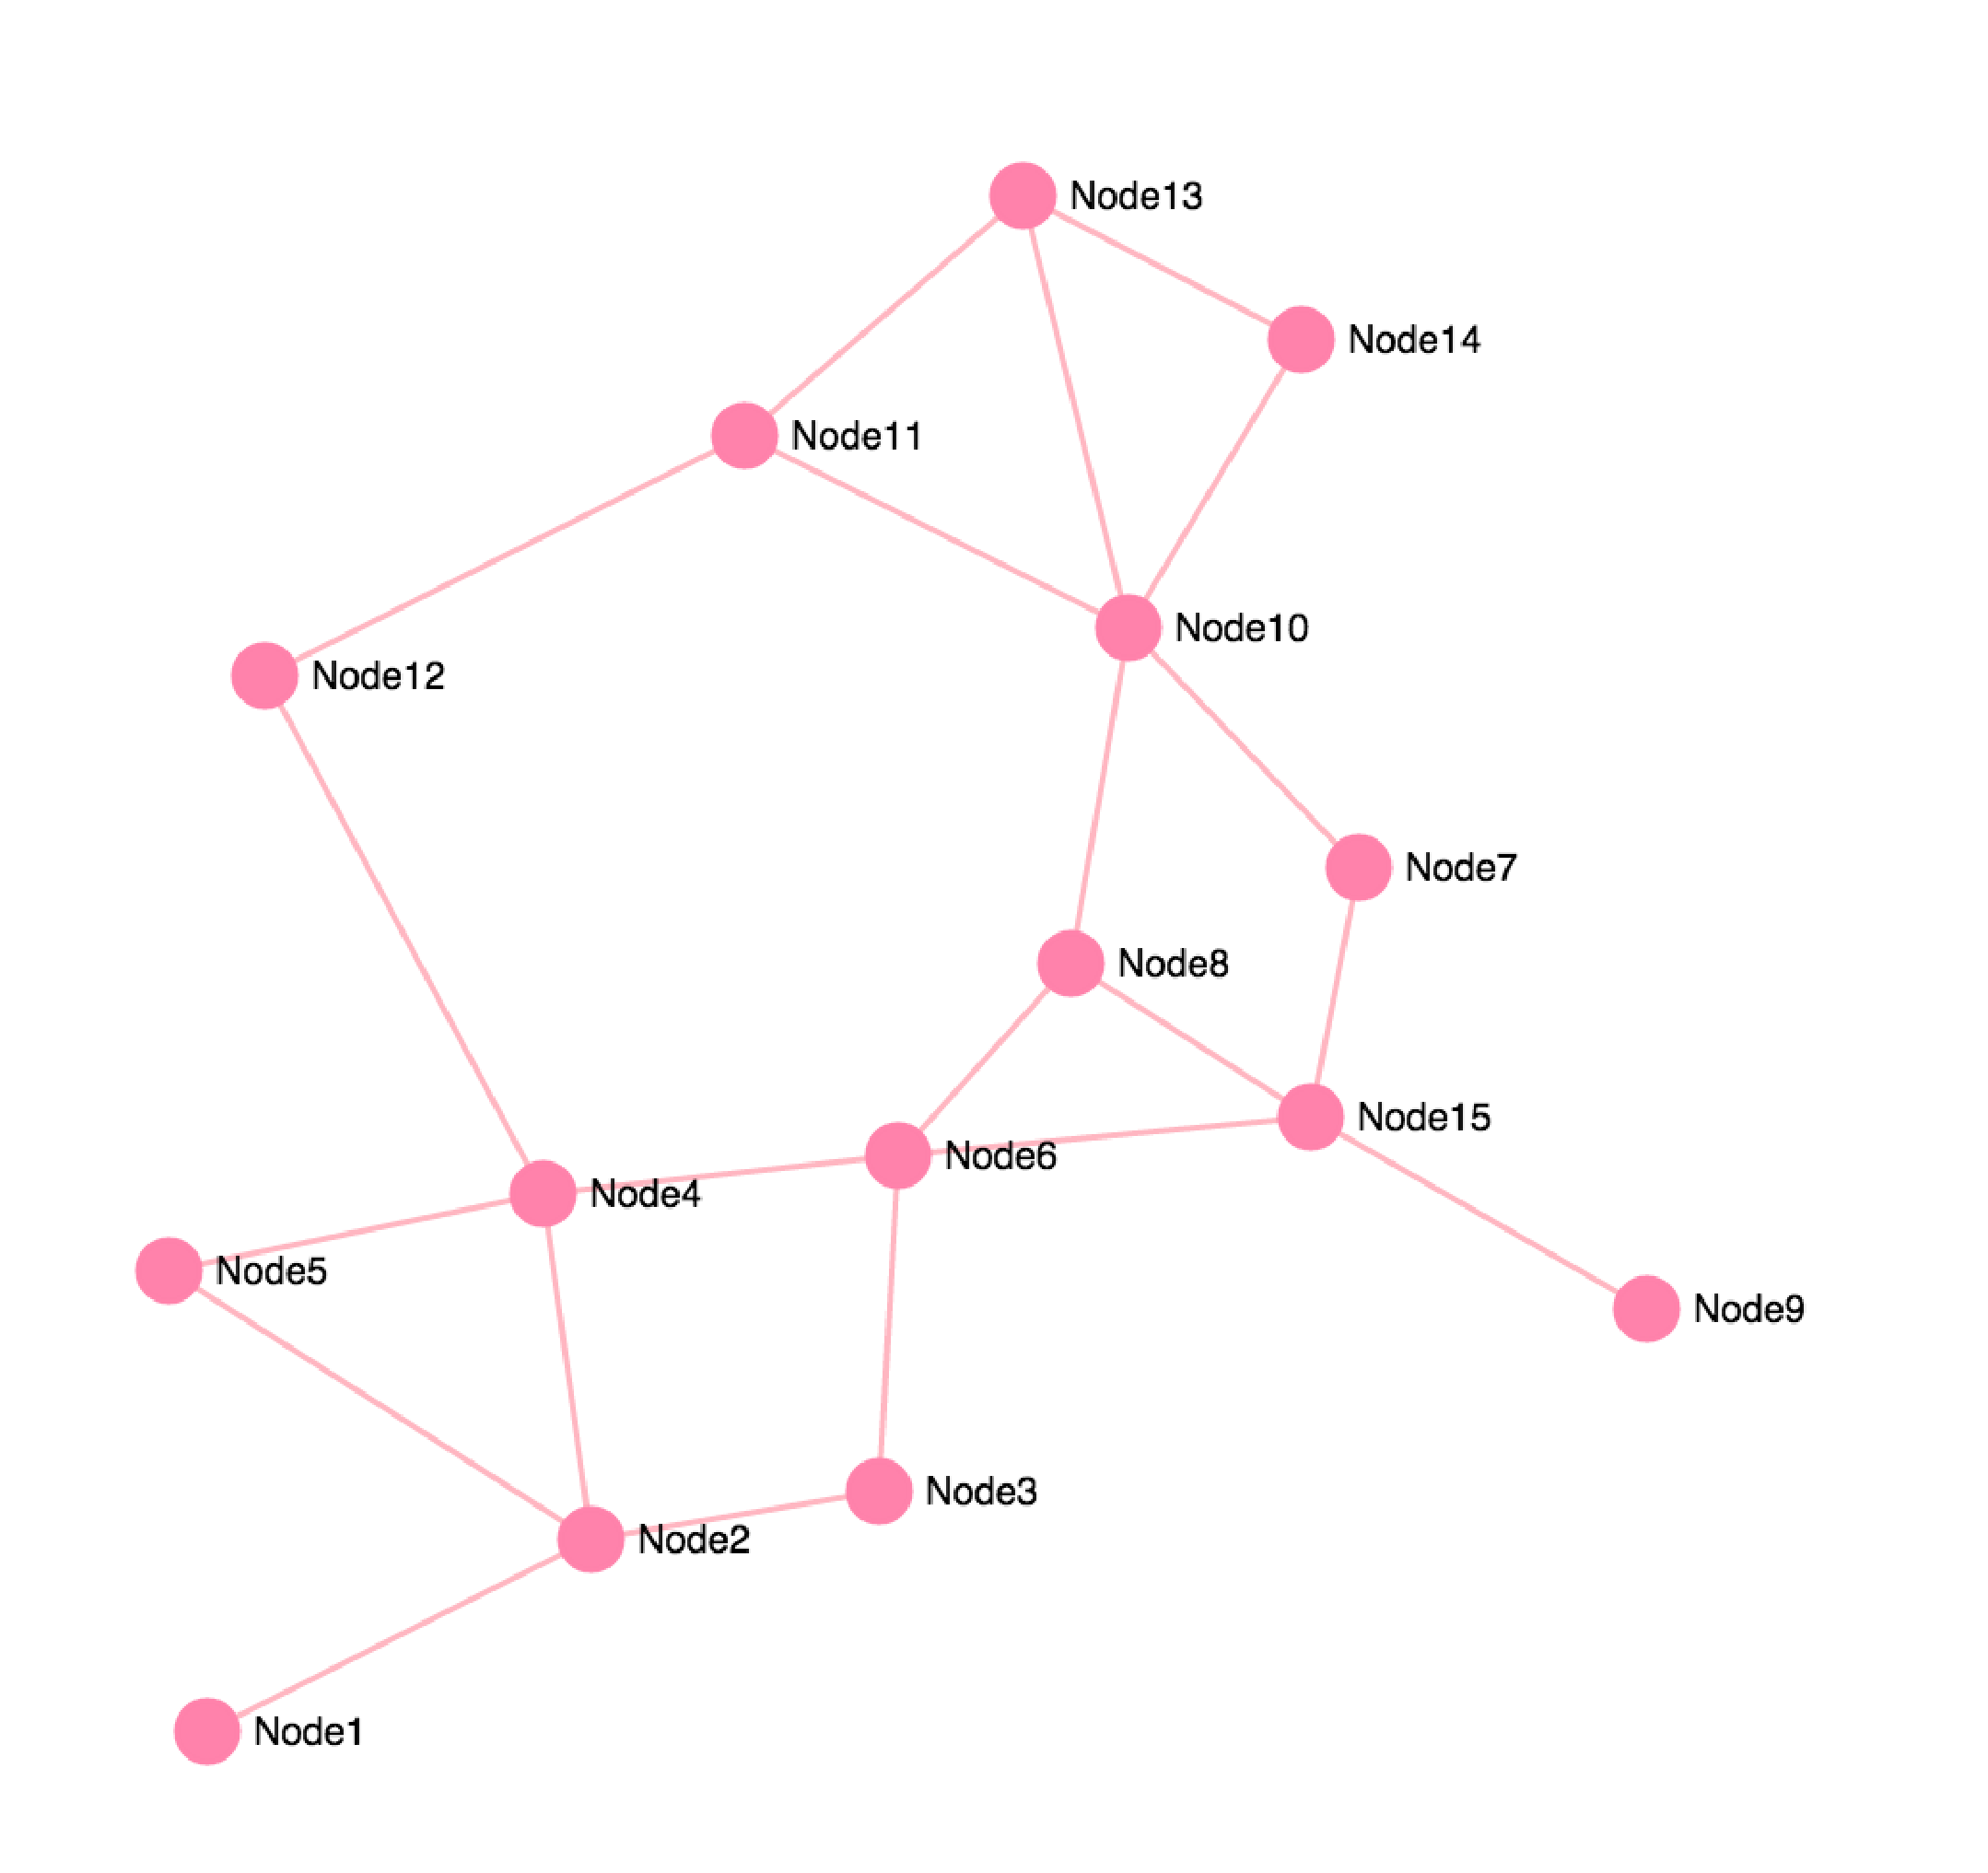
\includegraphics[width=4in]{assets/mandlnetwork_crop.png}
  \end{center}
  \caption{Illustration of Mandl's transit network as a graph}
  \label{fig:MandlNetwork_problemstatement} 
\end{figure}


